\section{Experiments with ChatGPT}
Over the last few years, Large Language Models (LLMs) such as GPT-3 \citep{gpt3} have achieved great amounts of success over a range of tasks in the NLP domain.

However, it has been shown that models such as ChatGPT struggle with mathematical and logical reasoning. 

\section{Temporal reasoning}

\section{Long LLM prompt}
\begin{quotation}
    \label{quote:long_prompt}
    Verbal aspect in language indicates how an action unfolds over time, emphasizing its internal structure, such as whether it is ongoing, completed, repeated, or momentary, distinct from tense which specifies when the action occurs relative to a reference point. The annotation distinguishes five base level aspectual values. The State value corresponds to stative events: no change occurs during the event. The Habitual value is annotated on events that occur regularly. The Activity value indicates an event with no inherent goal that has not necessarily ended and may be ongoing. Endeavor is used for processes which have an inherent end goal but which end without reaching completion (i.e., termination), whereas Performance is used for processes that reach a completed result state. Which class does "\emph{\{verb\}}" belong to in this sentence: state, habitual, activity, endeavor or performance?
\end{quotation}

\section{Annotation guidelines}
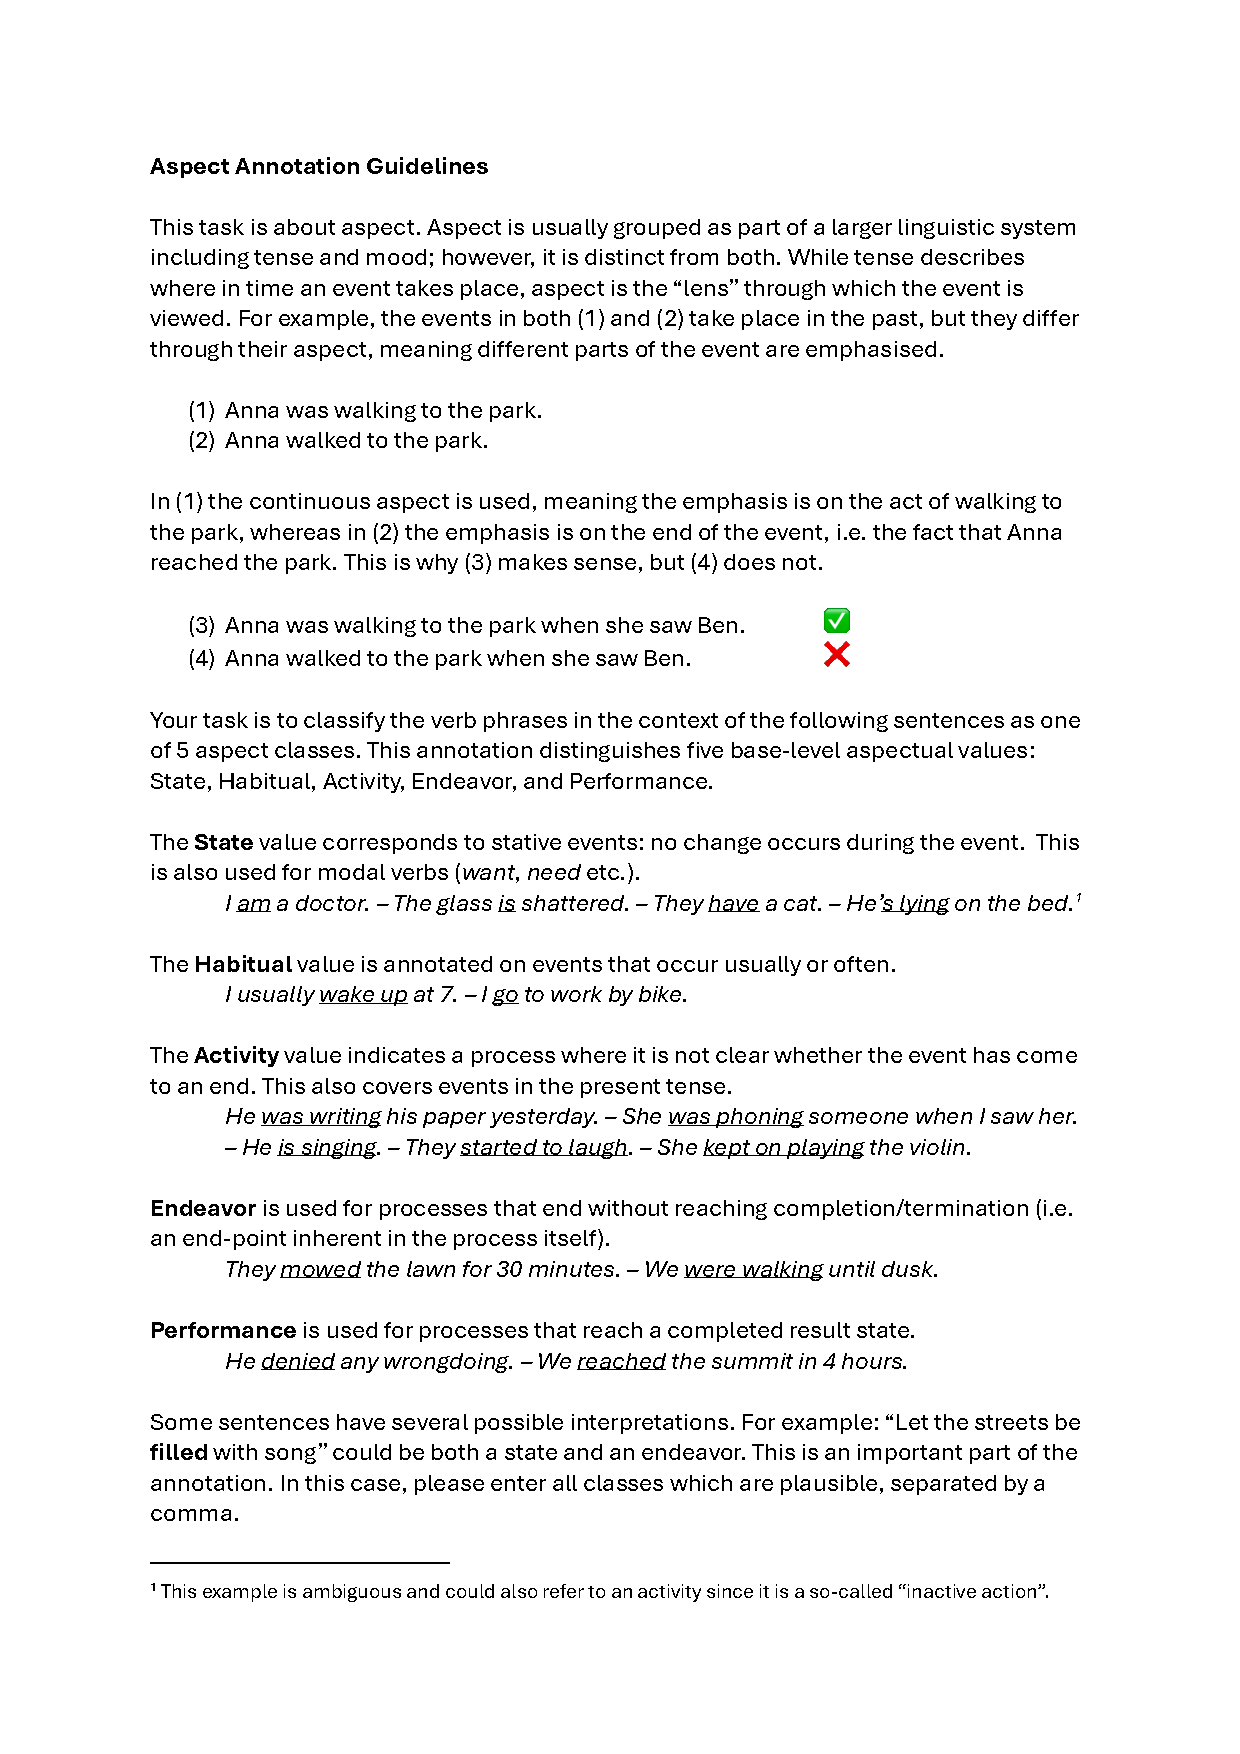
\includepdf[pages={-}]{img/ann_guide.pdf}
\label{App:annguide}

\section{Language-level entropy}
\label{App:lang_level_entropy_TED}
\begin{table}[ht]
    \centering
    \caption{Language-level Entropy on TED2013 dataset}
    \begin{tabular}{lcc}
        \toprule
        \textbf{Language} & \textbf{Mean Entropy} & \textbf{Variance} \\
        \midrule
        Chinese & $0.24579$ & $0.33647$ \\ \hline
        English & $0.32071$ & $0.19312$ \\
        German & $0.35085$ & $0.42130$ \\
        Dutch & $0.36985$ & $0.41680$ \\ \hline
        Italian & $0.36227$ & $0.42906$ \\
        Romanian & $0.33647$ & $0.40408$ \\
        Spanish & $0.36194$ & $0.43184$ \\
        Portuguese & $0.41209$ & $0.43718$ \\ \hline
        Polish & $0.31180$ & $0.41160$ \\
        Slovene & $0.29825$ & $0.38113$ \\
        Russian & $0.28984$ & $0.38741$ \\
        \bottomrule
    \end{tabular}
\end{table}

\begin{table}[ht]
    \centering
    \caption{Language-level Entropy on TED2020 dataset}
    \begin{tabular}{lcc}
        \toprule
        \textbf{Language} & \textbf{Mean Entropy} & \textbf{Variance} \\
        \midrule
        Arabic & $0.28453$ & $0.38861$ \\ \hline
        Vietnamese & $0.49336$ & $0.46466$ \\ \hline
        Chinese & $0.27207$ & $0.34002$ \\ \hline
        Danish & $0.43019$ & $0.42449$ \\
        Dutch & $0.36016$ & $0.41209$ \\
        English & $0.31668$ & $0.19319$ \\
        German & $0.34829$ & $0.42011$ \\
        Icelandic & $0.39461$ & $0.43853$ \\
        Norwegian Bokmål & $0.46367$ & $0.46847$ \\
        Norwegian Nynorsk & $0.42910$ & $0.46448$ \\
        Swedish & $0.42756$ & $0.46448$ \\ \hline
        Catalan & $0.45707$ & $0.48769$ \\
        French & $0.41091$ & $0.44966$ \\
        Italian & $0.36121$ & $0.42817$ \\
        Portuguese & $0.41012$ & $0.43479$ \\
        Romanian & $0.33490$ & $0.40521$ \\
        Spanish & $0.31668$ & $0.43953$ \\ \hline
        Estonian & $0.31668$ & $0.43953$ \\
        Finnish & $0.29564$ & $0.36784$ \\
        Hungarian & $0.32440$ & $0.39755$ \\ \hline
        Greek & $0.26212$ & $0.36320$ \\ \hline
        Latvian & $0.28655$ & $0.36055$ \\
        Lithuanian & $0.34829$ & $0.42011$ \\ \hline
        Belorussian & $0.28453$ & $0.38861$ \\
        Bulgarian & $0.28453$ & $0.38861$ \\
        Croatian & $0.27519$ & $0.37766$ \\
        Czech & $0.27519$ & $0.37766$ \\
        Polish & $0.30852$ & $0.40623$ \\
        Russian & $0.28529$ & $0.38692$ \\
        Slovakian & $0.28453$ & $0.38861$ \\
        Slovene & $0.28453$ & $0.38861$ \\
        Ukrainian & $0.24490$ & $0.35603$ \\
        \bottomrule
    \end{tabular}
\end{table}